\documentclass[a4paper, 11pt]{article}
\usepackage[left=2cm, top=3cm, text={17cm, 24cm}]{geometry}
\usepackage[czech]{babel}
\usepackage[utf8]{inputenc}
\usepackage[IL2]{fontenc}
\usepackage{times}
\usepackage{multirow}
\usepackage{array}
\usepackage{url}
\usepackage{graphics}
\usepackage[unicode, hidelinks, hyperfootnotes=false]{hyperref}
\usepackage{tikz}
\usepackage{pdflscape}
\usepackage[czech, linesnumbered, ruled, longend]{algorithm2e}
\newcommand{\condition}{$k = 1$ \KwTo $M$}

\urlstyle{same}
\author{Martin Valach//xvalac12@stud.fit.vutbr.cz}

\begin{document}
    \begin{titlepage}
		\begin{center}
			{\Huge\textsc{
			    Vysoké učení technické v~Brně
			    \\[0.2em]
			}
			\huge\textsc{
			    Fakulta informačních technologií
			}
			}
			\vspace{\stretch{0.382}}
			{\LARGE
				\\ Typografie a~publikování -- 3. projekt \\[0.3em]
				\Huge Tabulky a obrázky
			}
			\vspace{\stretch{0.618}}
		\end{center}

		{\Large
			\today
			\hfill Martin Valach
		}
	\end{titlepage}
	
	\section{Úvodní strana}
	Název práce umístěte do zlatého řezu a~nezapomeňte uvést \uv{dnešní} datum a vaše jméno a~příjmení.
	
	\section{Tabulky}
	Pro sázení tabulek můžeme použít buď prostředí\texttt{ tabbing }nebo prostředí\texttt{ tabular.}
	
	\subsection{Prostředí \texttt{ tabbing}}
	Při použití\texttt{ tabbing }vypadá tabulka nasledovně: 
	
	\begin{tabbing}
	    \verb|\pushtabs|\qquad \= \qquad \qquad\= \kill
    	\textbf{Ovoce} \> \textbf{Cena} \> \textbf{Množství} \\
	    Jablka \> 25,90 \> 3 kg \\
	    Hrušky \> 27,40 \> 2,5 kg \\
	    Vodní melouny \> 35,- \> 1 kus\\
	\end{tabbing}
    Toto prostředí se dá také použít pro sázení algoritmů, ovšem vhodnější je použít prostředí\texttt{ algorithm }nebo\texttt{ algorithm2e }(viz sekce \ref*{sec:alogoritmy}).
	
    \subsection{Prostředí \texttt{tabular}}
    Další možností, jak vytvořit tabulku, je použít prostředí\texttt{ tabular.} Tabulky pak budou vypadat takto\footnote{Kdyby byl problém s~\texttt{ cline}, zkuste sa podívat třeba sem: \url{http://www.abclinuxu.cz/tex/poradna/show/325037}.}:
    
    \begin{table}[h!] \catcode`\-=12
        \centering
        \begin{tabular}{| c | c | c |}
        \hline
         & \multicolumn{2}{| c |}{\textbf{Cena}}\\ \cline{2-3}
        \textbf{Měna} & \textbf{nákup} & \textbf{prodej} \\ \hline
        EUR & 24,775 & 25,943 \\
        GBP & 29,394 & 30,492 \\
        USD & 22,423 & 23,661 \\  
        \hline
    \end{tabular}
        \caption{Tabulka kurzů k dnešnímu dni}
        \label{table:tabulka1}
    \end{table}
    \medskip
    \begin{table}[ht!] \catcode`\-=12
        \centering
        \begin{minipage}{.11\linewidth}
        \begin{tabular}{| c | c |}
            \hline
            $A$ & $\neg A$ \\ \hline
            \textbf{P} & N \\ \hline
            \textbf{O} & O \\ \hline
            \textbf{X} & X \\ \hline
            \textbf{N} & P \\ 
            \hline
        \end{tabular}
        \end{minipage}%
        \begin{minipage}{.27\linewidth}
        \begin{tabular}{| c | c | c | c | c | c |}
        \hline
            \multicolumn{2}{|c|}{\multirow{2}{*}{$A \wedge B$}} & \multicolumn{4}{|c|}{$B$} \\ \cline{3-6}
            \multicolumn{2}{|c|}{} & \textbf{P} & \textbf{O} & \textbf{X} & \textbf{N} \\ \hline
            \multirow{4}{1em}{$A$} &\textbf{P} & P & O & X & N \\ \cline{2-6}
            &\textbf{O} & O & O & N & N \\ \cline{2-6}
            &\textbf{X} & X & N & X & N \\ \cline{2-6}
            &\textbf{N} & N & N & N & N \\ 
            \hline
        \end{tabular}
        \end{minipage}%
        \begin{minipage}{.27\linewidth}
        \begin{tabular}{| c | c | c | c | c | c |}
        \hline
            \multicolumn{2}{|c|}{\multirow{2}{*}{$A \vee B$}} & \multicolumn{4}{|c|}{$B$} \\ \cline{3-6}
            \multicolumn{2}{|c|}{} & \textbf{P} & \textbf{O} & \textbf{X} & \textbf{N} \\ \hline
            \multirow{4}{1em}{$A$} &\textbf{P} & P & P & P & P \\ \cline{2-6}
            &\textbf{O} & P & O & P & O \\ \cline{2-6}
            &\textbf{X} & P & P & X & X \\ \cline{2-6}
            &\textbf{N} & P & O & X & N \\ 
            \hline
        \end{tabular}
        \end{minipage}%
        \begin{minipage}{.3\linewidth}
        \begin{tabular}{| c | c | c | c | c | c |} 
        \hline
            \multicolumn{2}{|c}{\multirow{2}{*}{$A \rightarrow B$}} & \multicolumn{4}{|c|}{$B$} \\ \cline{3-6}
             \multicolumn{2}{|c|}{} & \textbf{P} & \textbf{O} & \textbf{X} & \textbf{N} \\ \hline
            \multirow{4}{1em}{$A$} &\textbf{P} & P & O & X & N \\ \cline{2-6}
            &\textbf{O} & P & O & P & O \\ \cline{2-6}
            &\textbf{X} & P & P & X & X \\ \cline{2-6}
            &\textbf{N} & P & P & P & P \\ 
            \hline
        \end{tabular}
        \end{minipage}
        \caption{Pretože Kleeneho trojhodnotová logika už je \uv{zastaralá}, uvádime si zde příklad čtyřhodnotové logiky} \label{table:tabulka2}
    \end{table}
    \medskip
    \pagebreak
    
    \section{Algoritmy} \label{sec:alogoritmy}
    Pokud budeme chtít vysázet algoritmus, můžeme použít prostředí\texttt{ algorithm}\footnote{Pro nápovědu, jak zacházet s prostředím\texttt{ algorithm,} můžeme zkusit tuhle stránku:\\ \url{http://ftp.cstug.cz/pub/tex/CTAN/macros/latex/contrib/algorithms/algorithms.pdf}.} 
    nebo\texttt{ algorithm2e}\footnote{Pro\texttt{ algorithm2 }zase tuhle: \url{http://ftp.cstug.cz/pub/tex/CTAN/macros/latex/contrib/algorithm2e/doc/algorithm2e.pdf}.}
    Príklad pro použití prostředí \texttt{ algorithm2e } viz Algoritmus \ref*{alg:algoritmus1}.
    
    
    \begin{algorithm}
        \SetAlgoNoLine
        \SetNlSty{}{}{:} 
        \SetKwInput{Input}{Input}
        \SetKwInput{Output}{Output}
        \Input{$(X_{t-1}, u_t, z_t)$}
        \Output{$X_t$}
        \BlankLine
        \SetNlSkip{-0.45cm}\Indpp\Indp\emph{$\overline{X_t} = X_t = 0$}\\
        \For{\condition}{
            \Indpp\emph{$x_t^{[k]} =$ sample\_motion\_model$(u_t,x_{t-1}^{[k]})$}\\
            \emph{$\omega_t^{[k]} =$ measurement\_model$(z_t,x_t^{[k]}, m_{t-1})$}\\
            \emph{$m_t^{[k]} =$ updated\_occupancy\_grid$(z_t,x_t^{[k]}, m_{t-1}^{[k]})$}\\
            $\overline{X_t} = \overline{X_t} + \langle x_x^{[k]},\omega_t^{[k]}\rangle$
        }
        \For{\condition}{
            \Indpp draw $i$ with probability $\approx \omega_t^{[i]}$\\
            add $\langle x_x^{[k]},m_t^{[k]}\rangle$ to $X_t$
        }
        \Return{$X_t$}
        \caption{\textsc{FastSLAM}}\label{alg:algoritmus1}
    \end{algorithm}
    
    \section{Obrázky}
    Do našich článků můžeme samozřejmě vkládat obrázky. Pokud je obrázkem fotografie, můžeme klidně použít bitmapový soubor. Pokud by to ale mělo být nějaké schéma nebo neco podobného, je dobrým zvykem takovýto obrázek vytvořit vektorově.
    
    \begin{figure}[!h]
        \centering
        \scalebox{0.4}{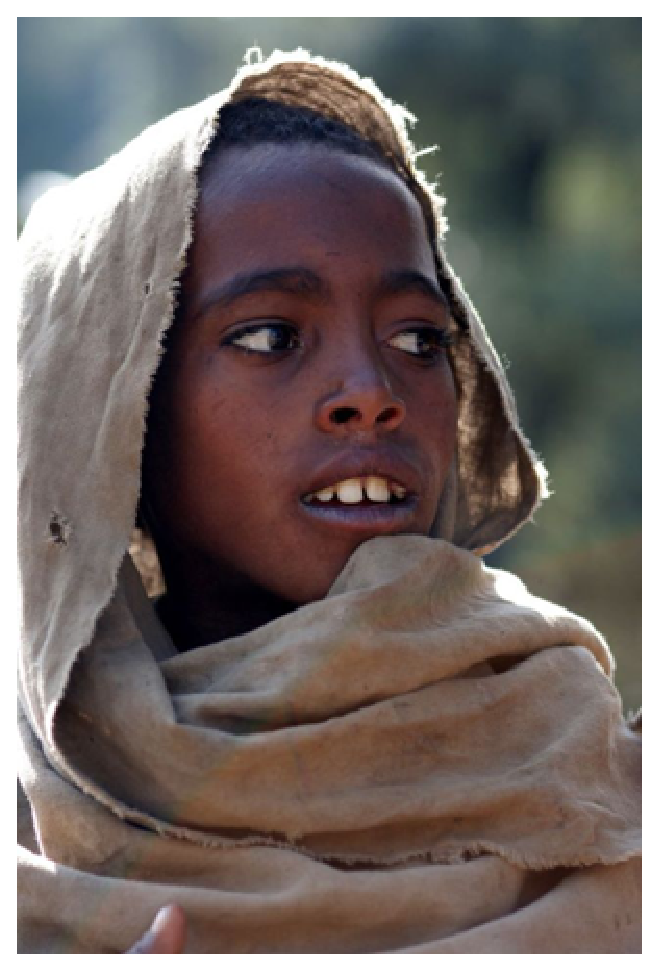
\includegraphics{etiopan.eps}\reflectbox{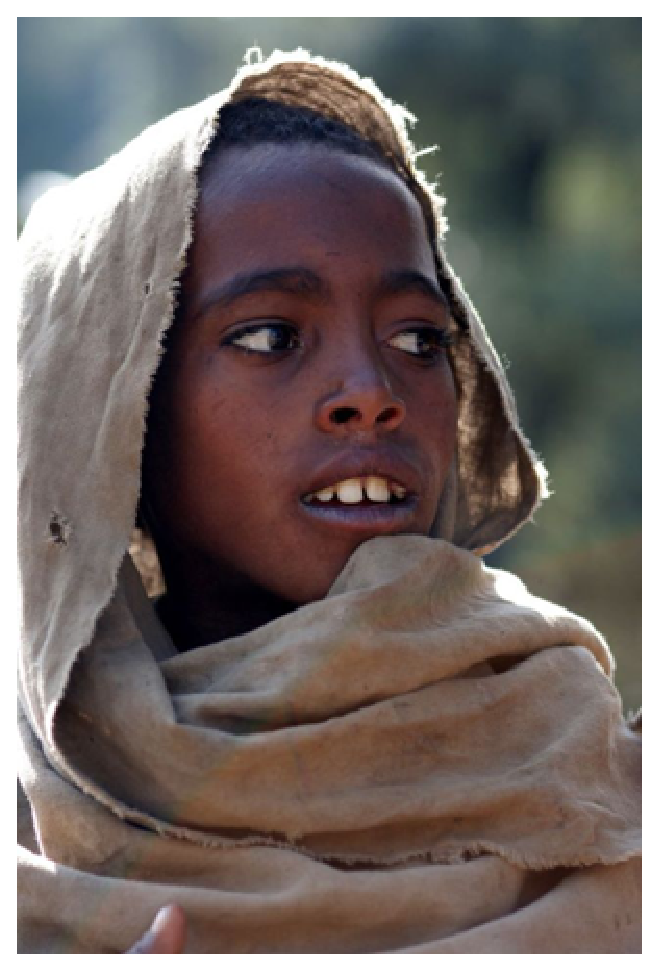
\includegraphics{etiopan.eps}}}
        \caption{Malý Etiopánek a jeho bratříček}
        \label{fig:obrazok1}
    \end{figure}
    
    
    \newpage
    Rozdíl medzi vektorovým \dots
    \begin{figure}[!h]
        \centering
        \scalebox{0.39}{
\includegraphics{oniisan.eps}}
        \caption{Vektorový obrázek}
        \label{fig:obrazok2}
    \end{figure}
    
    \dots a bitmapovým obrázkem
    \begin{figure}[!h]
        \centering
        \scalebox{0.58}{
\includegraphics{oniisan2.eps}}
        \caption{Bitmapový obrázek}
        \label{fig:obrazok3}
    \end{figure}
    
    \noindent se projeví například při zvětšení.
    
    Odkazy (nejen ty) na obrázky \ref*{fig:obrazok1}, \ref*{fig:obrazok2} a~\ref*{fig:obrazok3}, na tabulky \ref*{table:tabulka1} a~\ref*{table:tabulka2} a~také na algoritmus \ref*{alg:algoritmus1} jsou udělany pomocí křížových odkazů. Pak je ovšem je potřeba zdrojový soubor přeložit dvakrát.
    
    Vektorové obrázky lze vytvořit i~přímo v \LaTeX u, například pomocí prostředí\texttt{ picture}.
    
    \newpage
    \begin{landscape}
    \begin{figure}
        \centering
        \begin{tikzpicture}[scale=1.2]
            %zakladna struktura domu
            \draw[line width=10] (2.5,0) -- (2.5,0.1) -- (1,2) -- (6,3) -- (7.875,0.5) -- (13.5,0.5) -- (15,2.5) -- (10.5,2.5);
            \draw[line width=10] (6,3) -- (6,4) -- (15.5, 6);
            \draw (8.2, 0.7) -- (8.2, 4.6);
            \draw (10.5, 2.5) -- (10.5,5);
            
            %terasa
            \draw [very thick](13.5,3.2) -- (13.5, 5.7);
            \draw (10.5,3.2) -- (15.3, 3.2) -- (15.3, 2.7);
            \draw (10.5,3) -- (15.3, 3) -- (15.3, 2.7);
            \draw (10.5,2.8) -- (15.3, 2.8) -- (15.3, 2.7);
            
            \draw (12, 3.2) -- (12, 3.8) -- (13, 3.8) -- (13, 3.2) (12.5, 3.8) -- (12.5, 3.2); %dvere balkon
            \draw[color=black, fill=black!1, thick] (8.5,1.2) rectangle (10,2); %okno dolne
            \draw[color=black, fill=black!1, thick] (8.5,3) rectangle (10,3.8); %okno horne
            \draw[color=black, fill=black!1, thick] (12,1.2) rectangle (13,2); %okno dolne
            \draw[color=black] (10.5,0.6) -- (10.5,2) -- (11.5,2) -- (11.5,0.6) (11,0.6) -- (11,2); %dvere vchodove
            \filldraw[color=yellow!60, very thick](2,7) circle (1.2); %slnko
            \draw[black, very thick] (0,0) rectangle (19,8.5); %border
            \draw[color=black, very thick] (3,0) rectangle (6,1.5); %garazove dvere
            \draw (7,0) -- (7,0.3) -- (19,0.3) -- (19,0); %zaklady
            
            %virivka
            \draw[color=black, very thick] (15.6,0.3) rectangle (18,1.2);
            \draw (16.0,0.3) -- (16.0, 1.2);
            \draw (16.4,0.3) -- (16.4, 1.2);
            \draw (16.8,0.3) -- (16.8, 1.2);
            \draw (17.2,0.3) -- (17.2, 1.2);
            \draw (17.6,0.3) -- (17.6, 1.2);
            %\draw[color=black, fill=black!30, thick] (12,0.7) rectangle (13,2.3); %podperny stlp
        \end{tikzpicture}
        \caption{Vektorový obrázek moderního bydlení vhodného pro 21. století.}
        \label{fig:my_label}
    \end{figure}
    \end{landscape}
    
\end{document}